\documentclass[a4paper,12pt,oneside,pdflatex,italian,final,twocolumn]{article}

\usepackage[utf8]{inputenc}
\usepackage{parallel}
\usepackage{siunitx}
\usepackage{booktabs}
\usepackage{fancyhdr}
\usepackage{subcaption}
\usepackage{listings}
\usepackage{hyperref}
\usepackage{pdfpages}
\usepackage{smartdiagram}
\usepackage{verbatim}

\usepackage[export]{adjustbox}
\usepackage[margin=0.5in]{geometry}
\addtolength{\topmargin}{0in}

\usepackage{libertine}
\renewcommand*\familydefault{\sfdefault}
\usepackage[T1]{fontenc}

\urlstyle{sf}
\hypersetup{
	colorlinks=true, %set true if you want colored links
	linktoc=all,     %set to all if you want both sections and subsections linked
	linkcolor=blue,  %choose some color if you want links to stand out
	urlcolor=blue,   %url color
}

\smartdiagramset{text width=2cm,module x sep= 3.4,back arrow disabled=true,}

\title{Smarthome Measurement Node Prototype}
\author{Achmadi ST MT}
\date{April 2023}

\begin{document}
	\pagestyle{fancy}

	\lhead{VibrasticLab}
	\chead{\today}
	\rhead{Specification Document v1.0}

	\onecolumn

	\begin{figure}

	\end{figure}\begin{minipage}{0.47\textwidth}
		\centering

	\end{minipage}
	\hfill
	\begin{minipage}{0.47\textwidth}
		\raggedleft
		\Huge \textbf{Smarthome Measurement Node}
	\end{minipage}

	\begin{figure}
		\begin{minipage}{0.47\textwidth}

			\section{Overview}
			\begin{itemize}
				\item Battery AAA Operated
				\item Low-Power WiFi Cient
				\item Re-Programmable Firmware
				\item Analog, I2S, and I2C interfaces
				\item Indicator LEDs Array
			\end{itemize}


		\end{minipage}
		\hfill
		\begin{minipage}{0.47\textwidth}
			\centering
			\includegraphics[width=0.7\textwidth,right]{images/view_ortho.png}

	\end{minipage}
	\end{figure}

	\raggedright
	\section{Main Unit Part}

	\centering
	\begin{figure}[!ht]
		\centering
		\includegraphics[width=\textwidth,]{images/node_part.png}
		\caption{Prototype Unit Parts}
	\end{figure}

	\raggedright
	\section{Data Exchange Flow}

	\smartdiagram[flow diagram:horizontal]{Multi Sensor Node,
		MQTT or HTTP Server, Data Bank Server, Data Fetch API, Python or Matlab Analysis}\\

	\vspace{5pt}

	\textbf{NOTES:} Its recommended to use Local Server infrastructure, preferably in accessable server room during development phase.

	\raggedright
	\section{PCB Design}

	\newpage
	\includepdf[pages=-,angle=-90]{pdf/nodemcu_based.pdf}

	\newpage
	\includepdf[pages=-,angle=-90]{pdf/bom.pdf}

	\raggedright
	\section{Project Repository}

	Current project repository: \href{https://github.com/VibrasticLab/smarthome_proto}{Github VibrasticLab}

	\raggedright
	\section{Development Constraints/Obstacles}

	Some development constraints/obstacles:

	\begin{itemize}
		\item Time span, including: PCB building time, firmware implementation, testing and calibration, server building.

		\item Calibration process, including: standards, controlled test environment, and already available measurement tools.

		\item Personel requirement, including: programmers (either embedded or backend server), project managers/administrator, purchasing staff, etc.

		\item Components handling, for example:

		\begin{itemize}
			\item MG-811 CO2 sensor requires heating to operate, thus consume high power from battery.

			\item MG-811 CO2 sensor are very expensive and limited local stock.

			\item Light Intensity might influenced by placement angle.

			\item Mic INMP411 requires good digital signal processing in embedded programming manner.
		\end{itemize}

	\end{itemize}

	\raggedright
	\section{Cost Estimation}

	\subsection{Unit Cost}

	\begin{tabular}{|l|l|l|}
		\toprule
		Item & Price-Qty & URL \\
		\midrule
		NodeMCU ESP32 & Rp. 66.800 & \href{https://www.tokopedia.com/temins/esp32-esp-32-arduino-wifi-bluetooth-iot-development-board-micro-usb}{Tokped} \\
		HTU21D & Rp. 35.000 & \href{https://www.tokopedia.com/akhishop/htu21d-temperature-and-humidity-sensor-module}{Tokped} \\
		BH1750 & Rp. 20.000 & \href{https://www.tokopedia.com/akhishop/gy-302-light-intensity-bh1750-module-sensor-intensitas-cahaya}{Tokped} \\
		MG-811 CO2 & Rp. 895.000 & \href{https://www.tokopedia.com/khursiot/dfrobot-analog-co2-gas-sensor-for-arduino-mg-811-sensor}{Tokped} \\
		R 0805 & Rp. 2.000 & \href{https://www.tokopedia.com/thingie/resistor-0805-5-102-1k-ohm-smd-2012}{Tokped} \\
		LED 0805 & Rp. 2.000 & \href{https://www.tokopedia.com/easyware-id/led-smd-0805-super-bright-all-color-led-smd-0805-semua-warna-putih}{Tokped} \\
		Diode 1N4007 & Rp. 500 & \href{https://www.tokopedia.com/dx-tronics/diode-1n4007-in4007-dioda-rectifier-1a-1000v}{Tokped} \\
		Mic INMP411 & Rp. 40.000 & \href{https://www.tokopedia.com/aifrobotic/inmp441-omnidirectional-microphone-module-mems-i2s-interface}{Tokped} \\
		Header/Cable/Switches & Rp. 50.000 & \href{https://www.tokopedia.com/eltech-online}{Tokped} \\
		PCB Fabrication & Rp. 50.000 & \href{https://www.tokopedia.com/geraicerdas/cetak-pcb-1-keping-single-double-layer-rapid-prototyping-satuan}{Tokped} \\
		Shipping Cost Overall & Rp. 50.000 & - \\
		\midrule
		Total & Rp. 1.211.300  & - \\
		\bottomrule
	\end{tabular}

	\vspace{5pt}
	\textbf{Notes:} Its recommended to build multiple units to monitor single room in different multiple placements.

	\subsection{Personel Cost}

	\begin{tabular}{|l|l|l|l|}
		\toprule
		Jobs & Price & Personel & Alternative \\
		\midrule
		PCB Assembly and QC & Rp. 1.000.000 & Achmadi & Tim LabFisis \\
		Firmware Developer & Rp. 2.000.000 & Achmadi & Tim Labkom \\
		Purchasing Staff & Rp. 500.000 & - & Asisten LabVibrastik \\
		Project Manager/Admin & Rp. 1.000.000 & Ammar & Asisten LabVibrastik \\
		Calibration Team & Rp. 1.000.000 & - &  Asisten LabVibrastik \\
		Backend Developer & Rp. 2.000.000 & Pras & Tim Labkom \\
		Server Infastructure Team & Rp. 500.000 & - & Tim Labkom \\
		\midrule
		Total & Rp. 8.000.000  & - & - \\
		\bottomrule
	\end{tabular}

	\vspace{5pt}
	\textbf{Note:} This the recommended jobdesc list, but the price here are only proposed estimation and still negotiable.

	\subsection{Development Cost}

	\begin{tabular}{|l|l|l|}
		\toprule
		Item & Qty & Price \\
		\midrule
		Measurement Node Cost & 5 prototype units & Rp. 6.056.500 \\
		Personel/Team & one-time project & Rp. 8.000.000 \\
		\midrule
		Total & - & Rp. 14.056.500 \\
		\bottomrule
	\end{tabular}
\end{document}